\chapter{CNNs for computer vision}
\label{image-ann}

A paper Visualizing and Understanding Convolutional Networks by Matthew D. Zeiler and Robert Fergus \cite{zf-net} started with two sentences: \textit{Large Convolutional Network models have recently demonstrated impressive classification performance on the ImageNet benchmark. However there is no clear understanding of why they perform so well, or how they might be improved.}

I tried to disperse such clouds a bit in the previous chapter, but now I would like to focus on another undertone connected with those statements. On their applications in the computer vision.

Almost everything mentioned in chapter \ref{cnn} was already tied to the computer vision. The following text will briefly describe the field of computer vision itself and then introduce few tasks in that field connected with the topic of the thesis. In each task, few \zk{CNN} models will be mentioned. This text structure was chosen also to depict the models evolution concluding in the one selected for the practical part of this thesis - an implementation into GRASS GIS.

% different sizes

\section{Understanding computer vision}
\label{computer-vision}

When you see a group photo, you can easily count the number of people in the photo, you can say whether they are smiling or not, whether they are happy, sad, angry, you can even guess whether they are one family, a bunch of friends, colleagues or just random people passing by. You can do all of that in a fraction of a second without any effort. The computer vision is supposed to be a computer-aided version of this human cognition. Or in a fancier way, from \cite{opencv}: \textit{Computer vision is the transformation of data from a still or video camera into either a decision or a new representation.} The new representation might be for instance a colour shift, the decision an answer on a question like \textit{Is there any football field in the picture?}

However, the problem is that the claim that it is easy for humans does not mean that it is easy also for computers. As is generally known and was indicated in chapter \ref{understanding-cnn}, the human brain is an extremely complex tool. The other thing is that a computer receives a visual impulse (image) in other way as is illustrated in figure \ref{fig:mirror}. Where human sees a side mirror, a computer sees a grid of numbers. And this grid may be completely different when the daytime, viewpoint, brightness, background or scale changes.

\begin{figure}[H]
   \centering
	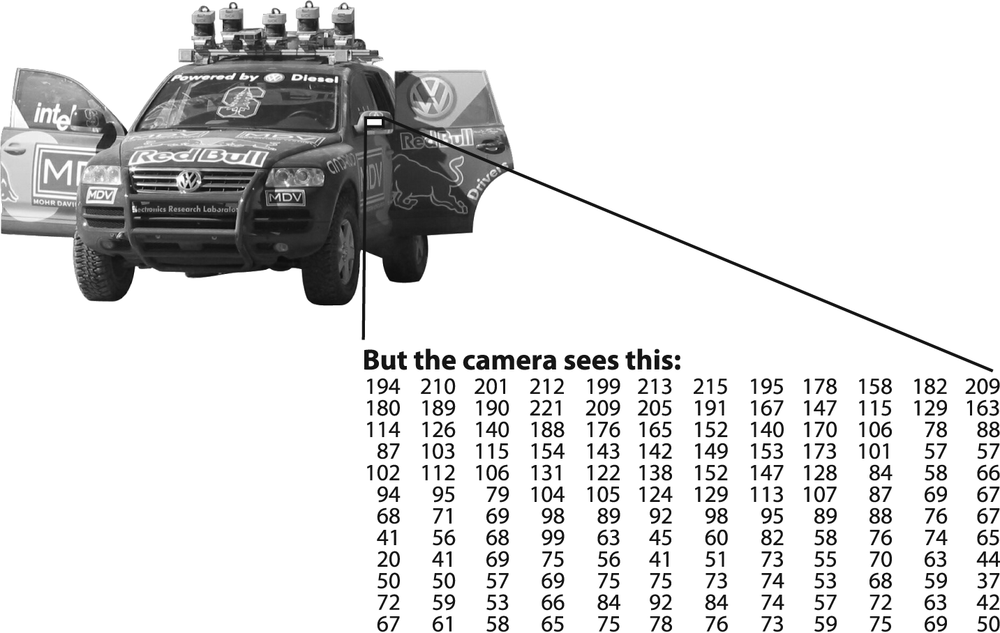
\includegraphics[width=.8\linewidth]{./pictures/comp-vision.png}
	\caption[Human and computer cognition]{The difference between human and computer cognition, source: \cite{opencv}}
      \label{fig:mirror}
\end{figure}

The task may be something like \textit{Is there any side mirror in the picture?} This kind of tasks can be seen in the field of computer vision daily and can be extremely difficult to solve in the computer way. Although the input may include some metadata, it still has to be solved in a strict mathematical way. And because our goal is to make our computer vision system \textit{perceive like a human}, it looks like the right place for \zk{CNN}s.

Although we will focus only on classification and connected tasks like detection and segmentation, there are many more applications of the computer vision. To name a few: Autonomous cars, face recognition, fingerprint recognition, motion capture, biometrics and remote sensing.

To get a better view into the field of computer vision, it is recommended to read a richer source like \cite{comp-vision} and \cite{opencv} to get some practice.

\section{Classification}
\label{classification}

The idea is simple, image classification is the task of assigning an image to one class. It means that the user is interested in the result of a guess of what the image contains. A good example are camera traps. When the user is interested in mooses, he can train his model to predict mooses and automatically filter all outputs from the camera trap through this validator.

The idea of training a model to sorting a list of numbers is quite straightforward. Due to differences in pictures of the same object caused by influences mentioned in chapter \ref{computer-vision}, the classification task needs a bit of oblique, but still strictly logical thinking. It needs a data-driven approach. Instead of defining how exactly should moose look like, we feed the model with a bunch of labeled examples. It is the same process as with human children.

However, the number of classes does not have to be equal to one. The user can have a set of multple classes and even his classifier may differ. A popular simple classifier is a binary classifier returning just 1 or 0 (representing True or False/Yes or no) for each class per image, but much more widely used one is a softmax function giving a vector of probabilities for classes. This classifier also somehow more represents the human mind, as we may be unsure if there is a moose or a wapiti in the picture, if it was taken with bad conditions.

\begin{figure}[H]
   \centering
	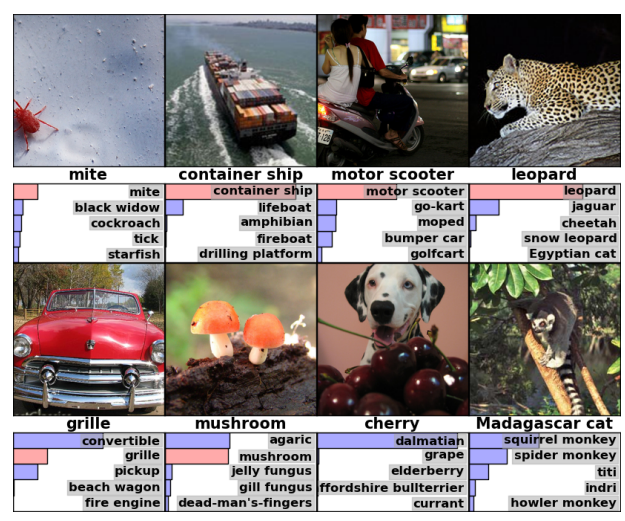
\includegraphics[width=.8\linewidth]{./pictures/classification.png}
	\caption[Classification example]{An example of the classification output with softmax function, source: \cite{cnn-classification}}
      \label{fig:class}
\end{figure}

The pioneering work in the field of \zk{CNN}-based classification is AlexNet proposed in \cite{cnn-classification} and described in chapter \ref{alexnet}. Another interesting implementation is the CNN-RNN framework for multi-label image classification\footnote{Real world images often contain more features; multi-label image classification tries to predict more than just one of them. The problem of one-label classification can be seen in the seventh image in figure \ref{fig:class}.} proposed in \cite{multi-classification}.

\section{Classification with localization}
\label{classification-localization}

Although classification with localization is sometimes ignored in similar lists as a subtype of object detection, I believe it is useful to mention it as a step between pure classification and object detection.

Classification was already explained in the previous chapter. Classification with localization uses classification in its one-class form together with bounding boxes (bounding boxes may be multiple). The goal is to draw the bounding box as tight around the object as possible and predict the class of the object, so the user ends up with two outputs:
\begin{itemize}
	\item \textbf{Class:} Class label
	\item \textbf{Bounding box:} Box in the image defined by two coordinates and its width and height.
\end{itemize}

Because multiple values are returned, this task can be considered as a kind of a regression problem. Outputs from the regression are enough to get a result as the one illustrated in figure \ref{fig:class-loc}. 

\begin{figure}[H]
   \centering
	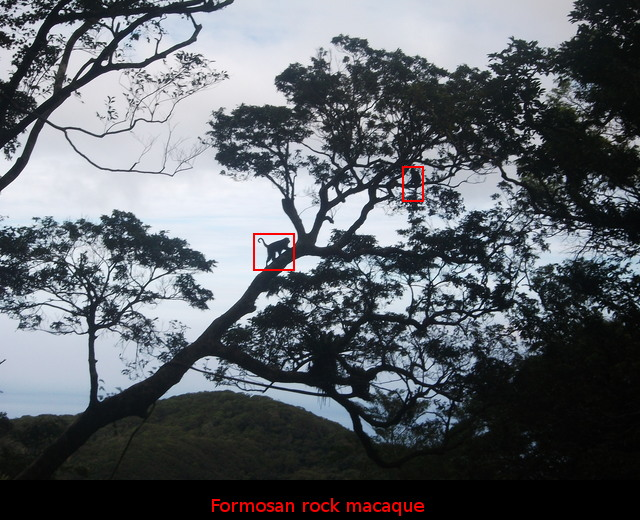
\includegraphics[width=.7\linewidth]{./pictures/class-loc.JPG}
	\caption[Classification with localization example]{An example of classification with localization}
      \label{fig:class-loc}
\end{figure}

\section{Object detection}
\label{object-detection}

% R-CNN, Fast, Faster
% Single-Shot MultiBox Detector (SSD) You Only Look Once (YOLO)

\section{Semantic segmentation}
\label{semantic-segmentation}

% CNN

\section{Instance segmentation}
\label{instance-segmentation}

% Mask R-CNN

% \section{Content-based Image Retrieval}